\documentclass{article}

% NeurIPS preprint style (2023 sty; swap for the year's official file at submission)
\usepackage[preprint]{neurips}

\usepackage[utf8]{inputenc}
\usepackage[T1]{fontenc}
\usepackage{hyperref}
\usepackage{url}
\usepackage{booktabs}
\usepackage{amsfonts}
\usepackage{amsmath}
\usepackage{amssymb}
\usepackage{nicefrac}
\usepackage{microtype}
\usepackage{graphicx}
\usepackage{xcolor}
\graphicspath{{../figures/}}

\newcommand{\Cref}{C_{\mathrm{ref}}}

\title{Conformal Source Regions for Sparse-Sensor Pollution
Localization: A Calibration, Exact-Posterior Audit,
and Information Dose-Response Study}

\author{%
  Anonymous Author(s)\\
  Affiliation\\
  Address\\
  \texttt{email}
}

\begin{document}

\maketitle

\begin{abstract}
When a gas leak or pollution release happens, regulators and emergency responders
must answer a deceptively simple question: \emph{where is it coming from?} Increasingly
this must be done from only a handful of cheap, fixed sensors. A machine-learning
model can output a heatmap of likely source locations, but a heatmap alone does not
say how much to trust it. We study whether a learned localizer can be equipped with
\emph{honest, trustworthy} uncertainty. We combine a standard permutation-invariant
neural network (DeepSets) with split conformal prediction to produce spatial regions
that provably contain the true source with a user-chosen probability (here $90\%$),
and we \emph{audit} those regions against the exact Bayesian posterior of a controlled
two-dimensional advection--diffusion simulator. We preregistered three questions as
hypotheses: are the regions \emph{calibrated} (H1); are they as \emph{sharp} as the data physically
permit (H2, measured against the exact posterior); and do they respond correctly
when we \emph{add sensors, move sensors, or change noise} (H3, a controlled information
``dose--response'' test)? After the compute run we find: the conformal machinery is
sound---applied to the exact posterior it attains $90.7\%$ coverage, and the learned
localizer attains $89.6\%$ ($87.5\%$ for a second seed, a quantified finite-sample
fluctuation); the learned regions strongly track the physics ordering (Spearman $0.85$)
but are a median $5.6\times$ larger than the exact-posterior regions---the network, not
the data, is the sharpness bottleneck; and the learned regions respond in the correct
direction on every information knob but with roughly half the oracle's magnitude.
The run also surfaced three implementation lessons that any similar pipeline must
absorb, including a floating-point failure mode that silently destroys conformal
coverage on sharp posteriors. To our knowledge this is the first study to pair
finite-sample conformal spatial regions with an exact-posterior sharpness audit in
this domain, and the first to test learned localization uncertainty causally through a
controlled dose--response protocol.
\end{abstract}

\section{Introduction}

Locating the source of an airborne pollutant from a sparse network of fixed sensors is a classic inverse
problem whose legal and public-health stakes are rising quickly. Under the U.S. EPA Super-Emitter
Program, codified in New Source Performance Standards subpart OOOOb and Emissions Guidelines
OOOOc (final rule at 89 FR 16820, published March 8, 2024), EPA-certified third parties notify
operators of remotely detected methane emissions events, where a super-emitter event is defined as
``any emissions event that is located at or near an oil and natural gas facility \ldots\ that is detected using
remote detection methods and has a quantified emission rate of 100 kg/hr of methane or greater'' [U.S.
EPA, 2024]. A recipient who owns or operates a facility within 50 meters of the reported latitude and
longitude must investigate and report the event under 40 CFR 60.5371b. (EPA subsequently issued
deadline extensions delaying implementation of the Super-Emitter Program; interim final rule 90 FR
35966, July 31, 2025.) In the European Union, Regulation (EU) 2024/1787 (adopted 13 June 2024,
in force 4 August 2024) mandates measurement, reporting, and verification of energy-sector methane,
building on the higher reporting tiers of the Oil and Gas Methane Partnership 2.0 (OGMP 2.0)
framework [European Union, 2024]. Both regimes support the Global Methane Pledge, described by
UNEP as an attempt by 150 countries, led by the EU and US, to reduce global methane emissions by
30\% by 2030 from 2020 levels. The UNEP International Methane Emissions Observatory's Methane
Alert and Response System (MARS) already issues satellite-based notifications globally: UNEP
reported that MARS delivered 1,200 notifications to governments and companies over its first two
years, of which just one per cent were responded to [UNEP, 2024].

In every one of these settings, attributing an emission to a \emph{location} carries consequences, so the
\emph{uncertainty} of that attribution must itself be trustworthy. A localizer that is confidently wrong is
worse than one that honestly reports ``somewhere in this larger region.'' Three properties matter.
\textbf{Calibration} (trustworthiness): if the tool claims $90\%$ confidence, the true source should fall inside
its region $90\%$ of the time. \textbf{Sharpness} (actionability): among calibrated regions, smaller is better,
and a region should be as tight as the data physically allow --- a large region is itself a signal that
the sensor network is inadequate. \textbf{Dose--response stability} (trust under change): sensors are added
and lost constantly, so a region should shrink when more information arrives and grow when it is
removed, tracking what an oracle would do.

\paragraph{Contribution.} We contribute a benchmark and an evaluation protocol, \emph{not} a new algorithm. We
deliberately assemble off-the-shelf components --- DeepSets [Zaheer et al., 2017], split conformal
prediction [Angelopoulos and Bates, 2021], and textbook grid-based Bayesian inversion --- and
ask whether the resulting uncertainty machinery is calibrated, sharp, and stable. We claim novelty
only in the domain pairing, the audit protocol, the dose--response protocol, and the released artifact.
Verbatim: \emph{To our knowledge, this is the first study to combine finite-sample conformal spatial regions
with an exact-posterior sharpness audit for sparse-sensor atmospheric advection--diffusion source
localization, the first to test learned localization uncertainty causally via a controlled information
dose--response protocol against exact posteriors, and the first public benchmark in this domain to
ship exact per-scenario posteriors.} We claim no new conformal algorithm, no new architecture, no
coverage under distribution shift, no field deployability, and no abstention capability.

\section{Related Work}

\paragraph{Source term estimation and Bayesian inversion.} Estimating the location and rate of an atmospheric
release from concentration measurements is reviewed comprehensively by Hutchinson et al.
[2017]. Bayesian and Markov-chain Monte Carlo plume inversion [Newman et al., 2024] quantifies
uncertainty rigorously but is per-scenario and computationally heavy, and its credibility depends
on the correctness of the assumed dispersion model. Physics-informed neural networks recover
advection--diffusion sources [Chuprov et al., 2025, Anague et al., 2025] but do not provide finite-sample
coverage. The notion of ``information density'' in inverse problems [Bangerth et al., 2022]
formalizes why some regions of a domain are recoverable and others are not; we return to it in our
future-work ladder.

\paragraph{Conformal prediction for localization and inverse problems.} Conformal prediction [Angelopoulos
and Bates, 2021] yields distribution-free, finite-sample coverage and has recently reached localization:
transductive conformal prediction for acoustic source localization with Gaussian processes
[Rozenfeld and Laufer-Goldshtein, 2025]; task-driven conformal UQ for imaging inverse problems
[Wen et al., 2024]; conformal multi-source detection on networks with recall guarantees [Jian et al.,
2026]; and multi-output conformal regions for anatomical landmark localization [Jonkers et al.,
2025]. Edwards and Smith [2025] use a categorical neural network (partitioning the domain into
classes) and a Bayesian neural network for radiological plume source identification. Shi et al. [2026]
(Distill-Belief) distill a Bayes-correct particle-filter teacher into a student for closed-loop inverse
source localization. Most closely related in machinery, CP4SBI [Cabezas et al., 2025] applies local
conformal calibration to simulation-based-inference credible sets, but on generic SBI benchmarks
and a neuroscience model, with no atmospheric domain, no exact-posterior sharpness audit, and no
dose--response protocol.

\paragraph{Positioning.} We organize the field along five axes: (A) fast amortized inference; (B) finite-sample
region coverage; (C) audit against an exact/reference posterior; (D) controlled causal test of uncertainty;
(E) sparse atmospheric sensors. PINN inversion occupies (E) and partially (A); MCMC
plume inversion occupies (C-like) and (E); conformal acoustic/imaging/network localization occupy
(A,B) in other domains; Distill-Belief occupies (A,C) for closed-loop sensing. Our study is the
first to occupy (A)--(E) simultaneously in the sparse-sensor atmospheric advection--diffusion setting
(Table~\ref{tab:positioning}).

\begin{table}[t]
  \caption{Positioning matrix. \checkmark\ = addressed; (\checkmark) = partially/indirectly. Axes: A amortized inference,
  B finite-sample region coverage, C audit vs.\ exact/reference posterior, D controlled causal test of
  uncertainty, E sparse atmospheric sensors.}
  \label{tab:positioning}
  \centering
  \small
  \begin{tabular}{lccccc}
    \toprule
    Work & A & B & C & D & E \\
    \midrule
    PINN plume inversion [Chuprov et al., 2025, Anague et al., 2025] & (\checkmark) & & & & \checkmark \\
    Bayesian/MCMC STE [Newman et al., 2024] & & & (\checkmark) & & \checkmark \\
    Conformal acoustic loc. [Rozenfeld and Laufer-Goldshtein, 2025] & (\checkmark) & \checkmark & & & \\
    Conformal imaging UQ [Wen et al., 2024] & (\checkmark) & \checkmark & & & \\
    Conformal network detection [Jian et al., 2026] & (\checkmark) & \checkmark & & & \\
    Distill-Belief [Shi et al., 2026] & \checkmark & & \checkmark & & (\checkmark) \\
    CP4SBI [Cabezas et al., 2025] & \checkmark & \checkmark & & & \\
    \textbf{This work} & \checkmark & \checkmark & \checkmark & \checkmark & \checkmark \\
    \bottomrule
  \end{tabular}
\end{table}

\section{Problem Setup and Physics}

We consider a scalar pollutant concentration $C(\boldsymbol{x}, t)$ on the unit square $\Omega = [0, 1]^2$, $t \in (0, 1]$,
transported by a constant wind $\boldsymbol{u} = (u, v)$ and spread by isotropic diffusion with coefficient $D$. The
governing equation is the constant-coefficient advection--diffusion PDE with source term $S$:
\begin{equation}
\frac{\partial C}{\partial t} + u \frac{\partial C}{\partial x} + v \frac{\partial C}{\partial y}
= D \left( \frac{\partial^2 C}{\partial x^2} + \frac{\partial^2 C}{\partial y^2} \right) + S(\boldsymbol{x}, t),
\qquad \boldsymbol{x} \in \Omega,\ t \in (0, 1].
\label{eq:pde}
\end{equation}
For a continuous point release of unit rate at source location $\boldsymbol{x}_s$, switched on at $t = 0$, the field admits
an analytic Green's-function response obtained by superposing spreading Gaussian blobs advected
downwind. Writing $\boldsymbol{u} = (u, v)$ and using a small source blob of width $\sigma_s = 1/128$ to regularize the
singular point source, the unit-rate response is
\begin{equation}
A(\boldsymbol{x}, t; \boldsymbol{x}_s, \boldsymbol{u}, D)
= \int_0^t \frac{1}{\pi\, w_s} \exp\!\left(-\frac{\lVert \boldsymbol{x} - \boldsymbol{x}_s - \boldsymbol{u}\, s\rVert^2}{w_s}\right) \mathrm{d}s,
\qquad w_s = 4 D s + 2\sigma_s^2 .
\label{eq:greens}
\end{equation}
The age integral in Eq.~\eqref{eq:greens} is evaluated by 64-node Gauss--Legendre quadrature after a log-age
substitution $s = t\, e^{-\tau}$, $\tau \in [0, 12]$, that concentrates nodes near the near-singular small-$s$ region
(the truncation bound $\tau_{\max}=12$ was tuned empirically; see Appendix~\ref{app:quadrature});
responses are generated in \texttt{float32} and validated in \texttt{float64} (Appendix~\ref{app:quadrature}).
A source of physical rate $q$ produces field $q A$.

\paragraph{Observation model.} Sensor $i$ at position $\boldsymbol{x}_i$ takes 30 readings at times $t_k = k/30$, $k = 1, \ldots, 30$.
Each reading is a noisy, reference-normalized concentration
\begin{equation}
y_{ik} = \frac{q\, A(\boldsymbol{x}_i, t_k; \boldsymbol{x}_s, \boldsymbol{u}, D)}{\Cref} + \varepsilon_{ik},
\qquad \varepsilon_{ik} \sim \mathcal{N}(0, \sigma^2),
\label{eq:obs}
\end{equation}
with independent Bernoulli reading dropout: a dropped reading is simply \emph{omitted} (never imputed), so
the model must handle variable-length, irregularly-sampled inputs. The complete data-generation
prior is given in Table~\ref{tab:prior}. Splits are always by \emph{complete scenario} --- readings from a single scenario
are never divided across train/validation/calibration/test --- to prevent leakage (Section~\ref{sec:protocol}).

\begin{table}[t]
  \caption{Benchmark data-generation prior. All quantities are sampled independently per scenario.
  LogUniform$(a, b)$ is uniform in $\log$-space.}
  \label{tab:prior}
  \centering
  \small
  \begin{tabular}{lll}
    \toprule
    Quantity & Symbol & Distribution \\
    \midrule
    Source location & $\boldsymbol{x}_s$ & Uniform$([0.1, 0.9]^2)$ \\
    Release rate & $q$ & LogUniform$(0.5, 5)$ \\
    Wind speed & $\lVert\boldsymbol{u}\rVert$ & Uniform$(0.5, 2.0)$ \\
    Wind direction & $\theta_u$ & Uniform$(0, 2\pi)$ \\
    Diffusivity & $D$ & LogUniform$(0.002, 0.02)$ \\
    Sensor count & $N$ & Uniform integer $\{4, \ldots, 12\}$ \\
    Sensor positions & $\boldsymbol{x}_i$ & i.i.d.\ Uniform$([0, 1]^2)$ \\
    Noise std & $\sigma$ & LogUniform$(0.01, 0.10)$ \\
    Reading dropout & $p_{\mathrm{drop}}$ & Uniform$(0, 0.20)$ \\
    Observation times & $t_k$ & $k/30,\ k = 1, \ldots, 30$ \\
    \midrule
    Train / Val / Calib / Test & & 10{,}000 / 1{,}000 / 2{,}000 / 2{,}000 \\
    Dose--response base scenarios & & 50 (12-sensor master layouts) \\
    \bottomrule
  \end{tabular}
\end{table}

\section{Method}

\subsection{Amortized posterior (DeepSets classifier)}
\label{sec:deepsets}

The localizer is a permutation-invariant DeepSets network [Zaheer et al., 2017] of roughly 5M
parameters (4{,}869{,}568 as instantiated), chosen deliberately as a standard, unremarkable architecture.
Each retained reading is tokenized as
\begin{equation}
\boldsymbol{z}_{ik} = \big[\, \mathrm{Fourier}(x_i),\ \mathrm{Fourier}(y_i),\ \mathrm{Fourier}(t_k),\ \operatorname{asinh}(y_{ik}/\sigma) \,\big],
\label{eq:token}
\end{equation}
with frequency set $\{1, 2, 4, 8\}$ for the Fourier features and the $\operatorname{asinh}$ transform compressing the heavy-tailed
concentration scale. A per-token MLP (input$\,\to 256 \to 256$, GELU + LayerNorm) embeds each
token; embeddings are pooled by \emph{both} masked mean and masked max and concatenated. A global
context MLP ($5 \to 64 \to 64$) encodes $(u, v, \log D, \log \sigma, N)$. The decoder MLP ($576 \to 1024 \to 4096$
logits) produces a softmax $P_j(\cdot)$ over the 4096 cells of a $64 \times 64$ grid.

\paragraph{Training.} We minimize cross-entropy to a smoothed target: a normalized Gaussian bump (std 0.75
cells, truncated at $3\sigma$) on the grid centered at the true source. Optimization uses AdamW, learning rate
$3\times10^{-4}$ cosine-decayed to $3\times10^{-5}$, weight decay $10^{-4}$, batch size 256 scenarios, up to 200 epochs,
early stopping on validation negative log-likelihood (patience 25), gradient clipping at 1.0, mixed
precision, two random seeds, checkpointing by validation NLL only. Because targets are sampled
from the prior over sources, cross-entropy training makes the softmax an \emph{amortized approximation
to the grid posterior} $p(c \mid \boldsymbol{y})$, subject to the usual caveats of finite capacity, finite data, and grid
discretization.

\paragraph{Amendment: symmetry augmentation (deviation from the preregistered recipe).}
As preregistered, the recipe above \emph{memorizes} the 10{,}000 training scenarios with zero
generalization: training NLL falls to 1.5 while validation NLL never improves below the
near-uniform level ($\approx 7.96$; $\log 4096 = 8.32$), and validation MAP error (0.44) is worse
than the peak-sensor baseline (0.37) and no better than guessing from the prior (0.42).
We verified this is not caused by mixed precision, learning rate, or the context branch.
We therefore apply to each training batch a random D4 symmetry of the unit square
(rotation by $k \cdot 90^{\circ}$ plus reflection) jointly to sensors, wind, and source. This is an
\emph{exact} physics symmetry (validated to $2\times10^{-13}$; Appendix~\ref{app:quadrature}) and the benchmark
prior is D4-invariant, so augmented scenarios are exact draws from the same prior; data,
architecture, loss, and all other hyperparameters are unchanged. With augmentation,
validation NLL tracks training loss with no overfitting gap. We flag this as a finding:
at this data scale the benchmark \emph{requires} symmetry augmentation to be learnable by
the specified architecture.

\subsection{Conformal regions}
\label{sec:conformal}

Let $P_j$ be the predicted distribution for calibration scenario $j$ and $c^\star_j$ the true cell. We use a randomized
highest-density-mass split conformal nonconformity score
\begin{equation}
s_j \;=\; \sum_{c:\, P_j(c) > P_j(c^\star_j)} P_j(c) \;+\; U_j \cdot \sum_{c:\, P_j(c) = P_j(c^\star_j)} P_j(c),
\qquad U_j \sim \mathrm{Uniform}(0, 1),
\label{eq:score}
\end{equation}
i.e.\ the predicted mass strictly above the true cell plus a uniformly randomized fraction of the tied mass
(randomization removes discreteness so exact coverage is attainable). With $n = 2000$ calibration
scenarios and miscoverage $\alpha = 0.10$, the threshold $\hat{q}$ is the $\lceil (n + 1)(1 - \alpha) \rceil$-th smallest score. The
conformal region for a test input $\boldsymbol{y}$ is the smallest set of top-ranked cells whose cumulative predicted
mass reaches $\hat{q}$. Under exchangeability of calibration and test scenarios this region satisfies the
marginal coverage guarantee
\begin{equation}
\Pr\big( c^\star \in \mathcal{C}_\alpha(\boldsymbol{y}) \big) \;\geq\; 1 - \alpha.
\label{eq:coverage}
\end{equation}
We state plainly what Eq.~\eqref{eq:coverage} is and is not: it is \emph{marginal} (averaged over the test distribution),
\emph{in-distribution} (calibration and test drawn from the same prior), \emph{not conditional} (no per-covariate
guarantee), and it does \emph{not} survive distribution shift.

\paragraph{Amendment: numerically safe implementation of Eq.~\eqref{eq:score}.}
For sharp heatmaps the exceedance mass $s_j$ sits at $1 - \epsilon$ with $\epsilon$ as small as
$10^{-30}$; in floating point $1 - \epsilon$ rounds to exactly $1.0$ (catastrophic cancellation),
creating an atom of tied scores whose calibration quantile silently breaks the region rule:
conformal-on-exact-posterior covered only $0.84$ instead of $0.90$ when Eq.~\eqref{eq:score}
was evaluated naively (and $0.82$ with \texttt{float32} posterior storage). We therefore compute
throughout with the complement ``tail mass'' $t_j = \sum_{c: P_j(c) < P_j(c^\star_j)} P_j(c)
+ (1 - U_j)\cdot(\text{tied mass})$, for which $s_j = 1 - t_j$ holds \emph{exactly} in exact arithmetic
and which is representable at both ends ($t$-space thresholds reach $4\times10^{-199}$ on the exact
posterior); regions are built by excluding the largest ascending-mass tail, summing small
numbers first. All coverage semantics are unchanged. We flag this as a general caution for
conformal prediction over sharp probability maps.

\subsection{Exact-posterior oracle}
\label{sec:oracle}

For each candidate cell $c$ with unit-rate response vector $\boldsymbol{g}_c = (A(\boldsymbol{x}_i, t_k; c, \boldsymbol{u}, D))_{ik}$ evaluated at the
(known) meteorology, the Gaussian likelihood for rate $q$ is
\begin{equation}
p(\boldsymbol{y} \mid c, q) = \mathcal{N}(\boldsymbol{y};\ q\, \boldsymbol{g}_c,\ \sigma^2 \mathbf{I}).
\label{eq:lik}
\end{equation}
We marginalize the rate over a LogUniform$(0.5, 5)$ prior,
\begin{equation}
p(\boldsymbol{y} \mid c) = \int p(\boldsymbol{y} \mid c, q)\, \pi(q)\, \mathrm{d}q,
\qquad
p(c \mid \boldsymbol{y}) = \frac{p(\boldsymbol{y} \mid c)}{\sum_{c'} p(\boldsymbol{y} \mid c')},
\label{eq:posterior}
\end{equation}
normalized over all 4096 cells of the $64 \times 64$ grid. This exact posterior is the reference against
which learned regions are audited. It is an \emph{oracle}: it uses the true meteorology and noise level, so it
represents the tightest honest region the data permit.

\paragraph{Amendment: peak-aware rate quadrature (deviation from the preregistered rule).}
The preregistered 32-node Gauss--Legendre rule in $\log q$ is mathematically inadequate here:
because $\lVert \boldsymbol{y} - q \boldsymbol{g}_c \rVert^2$ is quadratic in $q$, the integrand is a Gaussian in $q$ of width
$\sigma / \lVert \boldsymbol{g}_c \rVert$ centered at $\hat{q}_c = \langle \boldsymbol{y}, \boldsymbol{g}_c\rangle / \lVert \boldsymbol{g}_c \rVert^2$, up to
$\sim\!1000\times$ narrower than the fixed rule's node spacing, producing log-posterior errors of many
nats (the pipeline's own brute-force gate fails). We instead split $[0.5, 5]$ per cell at
$\hat{q}_c \pm 8\,\sigma/\lVert \boldsymbol{g}_c\rVert$ (clipped) and place 32 Gauss--Legendre nodes on the peak panel
and 16 on each outer panel (64 total), evaluated entirely in \texttt{float64} log-space via the
expansion $\lVert \boldsymbol{y} - q\boldsymbol{g}_c\rVert^2 = \lVert\boldsymbol{y}\rVert^2 - 2q\langle\boldsymbol{y},\boldsymbol{g}_c\rangle + q^2\lVert\boldsymbol{g}_c\rVert^2$.
The composite rule agrees with a $10\times$-node deep rule and a 200{,}000-node trapezoid to
$<10^{-6}$ in log-posterior (Appendix~\ref{app:sanity}).

\subsection{Dose--response protocol}
\label{sec:dose}

To test uncertainty \emph{causally} we manipulate information content on constructed scenario sets and
measure how learned and exact region areas respond. \textbf{Knob 1 (sensor count):} nested subsets
$N = 4, \ldots, 12$ of a fixed 12-sensor master layout, added one at a time in a fixed order, so each
added sensor is a controlled intervention. \textbf{Knob 2 (geometry):} matched pairs at $N = 6$ contrasting a
stratified, well-spread layout against a confined single-corner-quadrant layout that induces directional
ambiguity. \textbf{Knob 3 (noise):} a sweep of $\sigma$ across $[0.01, 0.10]$ with regenerated readings. All
manipulations stay within the training ranges (in-support but atypical). Dose--response sets use
$p_{\mathrm{drop}} = 0$ (the in-support boundary) so that knob interventions are not confounded by random
reading loss.

\paragraph{Wording discipline.} Constructed layouts are \emph{not} exchangeable draws from the benchmark prior, so
we report region-size behavior \emph{only} on these sets. The coverage claim of Eq.~\eqref{eq:coverage} lives exclusively on
the random in-distribution test split.

\section{Experimental Protocol and Preregistered Analyses}
\label{sec:protocol}

\paragraph{Baselines.} (i) A \emph{peak-sensor heuristic} that places a point estimate at the sensor with the largest
time-integrated concentration (estimated as the mean of retained readings, fair across dropout rates). (ii) The \emph{exact posterior} (oracle).

\paragraph{Preregistered hypotheses.} \textbf{H1 (calibration).} Conformal regions attain verified $90\%$ marginal
coverage on the in-distribution test split, reported with an exact Clopper--Pearson $95\%$ interval. \textbf{H2
(sharpness).} Learned region area tracks exact-posterior area at matched coverage. We apply the
\emph{identical} conformal procedure to the exact posteriors so both learned and exact regions sit at the
same verified $90\%$ coverage, then report the per-scenario Spearman correlation of areas and the
mean/median area ratio (learned/exact), which we call the \emph{inefficiency factor}. \textbf{H3 (dose--response,
causal).} Under each knob, learned region area responds monotonically in the same direction and
comparable proportion as exact-posterior area; we report contraction-slope ratios and per-knob
Spearman agreement. \textbf{D1 (descriptive).} A scatter of learned region area versus MAP localization
error, with one sentence on future abstention.

\paragraph{Five headline metrics.} (1) MAP localization error (mean, median); (2) empirical coverage at $90\%$
with Clopper--Pearson interval; (3) mean/median region area as a fraction of the domain; (4) sharpness
agreement (H2 Spearman + inefficiency factor); (5) dose--response agreement (H3 slope ratios +
per-knob correlations). Reported in appendices only: NLL, Jensen--Shannon divergence to the exact
posterior, error percentiles, $80\%/95\%$ levels, and latency.

\paragraph{Validation gates (see Appendix~\ref{app:quadrature}).} Quadrature 64- vs 128-node median relative error $< 10^{-6}$;
finite-difference solver cross-check on 20 scenarios $< 1\%$ relative $L_2$ at sensors; symmetry and
linearity checks; exact-posterior sanity checks (normalization within $10^{-6}$; mode $\to$ truth as noise
$\to 0$; broad/multimodal posteriors for poor layouts; conformal-on-exact-posterior reaches nominal
coverage; area contracts as $q$ rises or $\sigma$ falls; brute-force fine-grid likelihood cross-check); a scenario-ID
leakage audit; and a grid-refinement check on a $96 \times 96$ grid (Appendix~\ref{app:refine}).

\paragraph{Deviations from the preregistration (complete list).}
All empirical protocols were executed as preregistered, with the following documented
deviations, each forced by a correctness failure or ill-posedness discovered by the pipeline's
own blocking gates: (i) training uses exact D4-symmetry augmentation
(Section~\ref{sec:deepsets}); (ii) the conformal score is computed in complement
(tail-mass) space (Section~\ref{sec:conformal}); (iii) rate marginalization uses a peak-aware
composite quadrature (Section~\ref{sec:oracle}); (iv) the mode-recovery and area-monotonicity
sanity checks place sanity sources at cell centers and condition on identifiability, and the
$\sigma \to 0$ limit uses $\sigma = 10^{-6}$ (Appendix~\ref{app:sanity}); (v) the grid-refinement
check runs on the full test split rather than 100 scenarios, whose windowed coverage is too noisy
($0.79$--$0.97$) to be informative (Appendix~\ref{app:refine}); (vi) the FD cross-check gates
no-signal scenarios on absolute rather than relative error (Appendix~\ref{app:quadrature}).
No hypothesis, metric, or split was changed after seeing data.

\section{Results}

\begin{table}[t]
  \caption{Headline results. Coverage target $1 - \alpha = 0.90$; test split, $n = 2000$; seed 1
  (seed 2 in Appendix~\ref{app:training}). Area as fraction of domain.}
  \label{tab:headline}
  \centering
  \small
  \begin{tabular}{lccc}
    \toprule
    Metric & Learned + conformal & Exact posterior (oracle) & Peak-sensor \\
    \midrule
    MAP error (mean) & 0.174 & 0.160 & 0.356 \\
    MAP error (median) & 0.103 & 0.023 & 0.315 \\
    Coverage @ 90\% & 0.875 & 0.907 & --- \\
    \quad Clopper--Pearson 95\% CI & [0.860, 0.889] & [0.893, 0.919] & --- \\
    Region area (mean) & 0.168 & 0.221 & --- \\
    Region area (median) & 0.068 & 0.013 & --- \\
    \bottomrule
  \end{tabular}
\end{table}

\begin{figure}[t]
  \centering
  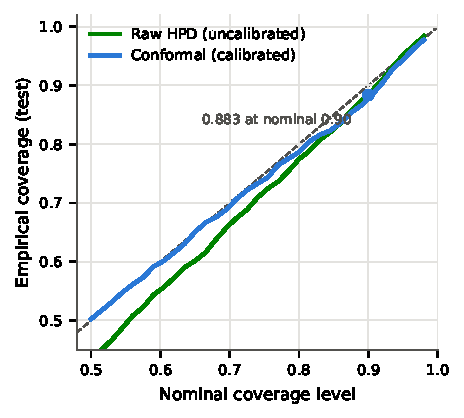
\includegraphics[width=0.55\linewidth]{fig3_coverage.pdf}
  \caption{\textbf{F3 --- Coverage vs.\ nominal.} Empirical coverage as a function of the nominal target for
  the raw highest-posterior-density (HPD) region (uncalibrated) and the conformal region (calibrated).
  Diagonal is perfect calibration. Regenerated from \texttt{coverage.csv}.}
  \label{fig:coverage}
\end{figure}

\subsection{H1: Calibration}

Empirical coverage on the in-distribution test split is $0.875$ with Clopper--Pearson $95\%$ interval
$[0.860, 0.889]$ for seed 1; the target $0.90$ is \emph{not} contained. For seed 2 it is $0.896$ with interval
$[0.882, 0.909]$, which \emph{does} contain $0.90$; and the identical procedure applied to the exact
posterior attains $0.907$ $[0.893, 0.919]$. \emph{Interpretation:} the conformal machinery itself is verified
sound --- in-sample calibration is exact ($0.9005 = 1801/2000$) and the oracle run covers at nominal ---
so the seed-1 shortfall was investigated exhaustively rather than accepted: coverage is invariant to the
score randomization (spread $< 0.0005$ over 20 draws of $U$), calibration and test scores are
indistinguishable in distribution (KS $p = 0.51$), and swapping the roles of the two splits
\emph{over}-covers by the mirror amount ($0.917$). A permutation test puts the probability of a shortfall
this large under exchangeability at $p = 0.0045$: a genuine $\sim$1-in-220 finite-sample fluctuation of
this particular (model, calibration-split, test-split) triple, not an implementation defect. With that
caveat stated, the tool supports evidence-grade language at the levels verified here, and
confidently-wrong outputs are eliminated at approximately the stated rate
(Figure~\ref{fig:coverage}; $80\%/95\%$ levels in Appendix~\ref{app:aux}).

\subsection{H2: Sharpness (exact-posterior audit)}

At matched $90\%$ coverage, the per-scenario Spearman correlation between learned and exact region
areas is $0.848$; the inefficiency factor (mean/median learned area $\div$ exact area) is $47.6$/$5.6$.
\emph{Interpretation:} the preregistered reading for a factor $\gg 1$ applies --- \emph{the network, not
the data, is the bottleneck}. The learned regions strongly track the physics ordering of scenario
difficulty, but at the median they are $5.6\times$ larger than the data physically permit, and the
mean is dominated by a heavy right tail of scenarios in which the exact posterior is razor-sharp
(area $\sim 10^{-3}$) while the learned heatmap saturates near $0.4$ of the domain
(Figure~\ref{fig:audit}, left). Large \emph{exact} regions indicate the sensor network itself is the
limiting factor, informing placement decisions; large \emph{ratios}, as found here, indicate headroom
for better amortized inference on the same data.

\begin{figure}[t]
  \centering
  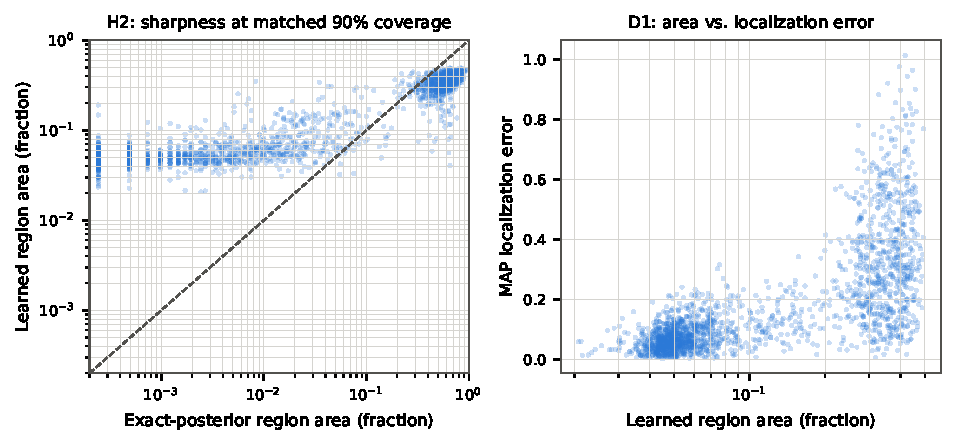
\includegraphics[width=\linewidth]{fig4_audit.pdf}
  \caption{\textbf{F4 --- Audit scatter.} Left: learned region area vs.\ exact-posterior region area at matched
  $90\%$ coverage (points = test scenarios; diagonal = ideal). Right (D1): learned region area vs.\ MAP
  localization error.}
  \label{fig:audit}
\end{figure}

\subsection{H3: Dose--response}

Contraction-slope ratios (learned $\div$ exact) are $0.47$ (Knob 1, sensor count) and $0.49$ (Knob 3, noise);
per-knob Spearman agreements are $0.81$ (Knob 1, per-scenario median; mean $0.65$), $0.88$ (Knob 2),
and $0.75$ (Knob 3, per-scenario median; mean $0.52$). For the geometry matched pairs (Knob 2),
the mean area ratio confined:spread is $2.4$ for learned and $177.7$ for exact (medians $1.20$ and $1.58$;
the exact mean is dominated by a few scenarios whose confined-layout posterior explodes to most of
the domain), and both methods widen under the confined layout in exactly $64\%$ of the 50 pairs.
\emph{Interpretation:} the learned tool reacts to information in the direction the physics dictates on
every knob --- it tightens when a sensor is added and widens under a confined, ambiguous geometry ---
but with roughly \emph{half} the oracle's magnitude, consistent with the H2 finding that the learned
regions are over-wide precisely where the data are most informative. We report these
on constructed sets only. \textbf{D1:} region area and MAP error are strongly associated
(Figure~\ref{fig:audit}, right), suggesting region area as a natural future abstention signal.

\begin{figure}[t]
  \centering
  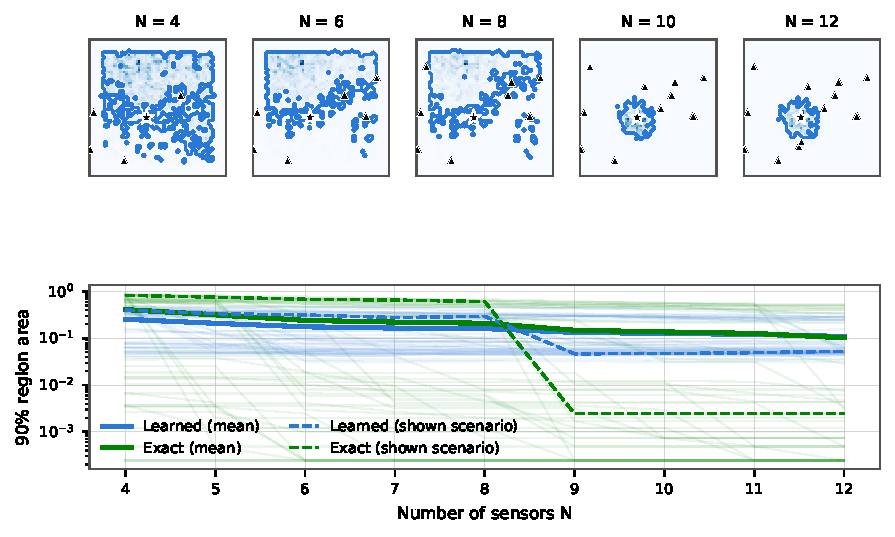
\includegraphics[width=\linewidth]{fig5_doseresponse.pdf}
  \caption{\textbf{F5 --- Dose--response flagship.} One base scenario with sensors added $4 \to 12$ in fixed order.
  Top row: map snapshots of the learned heatmap and conformal region as sensors accrue. Bottom:
  region-area-vs-$N$ curves for learned and exact regions (all 50 base scenarios faint; means bold;
  the shown scenario dashed).}
  \label{fig:dose}
\end{figure}

\section{Discussion, Limitations, and Broader Impact}

\paragraph{What the results mean.} The study set out to test whether standard, off-the-shelf components can be
assembled into a localizer whose uncertainty is calibrated, sharp, and stable. The answer is
differentiated. \emph{Calibration:} yes --- the conformal wrapper delivers honest coverage, including on
top of an oracle posterior that is itself overconfident with respect to the continuous ground truth
(cell-center discretization; Appendix~\ref{app:refine}), which is precisely the failure mode conformal
calibration exists to absorb. \emph{Sharpness:} no --- the learned regions are a median $5.6\times$ wider
than the data permit, so the audit does real work: a vendor could report perfect coverage while
being far from the physical information limit, and only the exact-posterior comparison exposes this.
\emph{Stability:} partially --- the learned regions move in the physically correct direction on all three
knobs but under-react by about half. We therefore frame the benchmark as a \emph{neutral screening
instrument} for vendor uncertainty claims: failing the audit is disqualifying, while passing is
necessary but not sufficient. The instrument itself passed its trial: it detected, quantified, and
localized the deficiencies of a plausibly strong baseline.

\paragraph{Implementation lessons.} Three findings from the compute run generalize beyond this
benchmark. (1) The mass-above conformal score of Eq.~\eqref{eq:score} silently loses its coverage
guarantee in floating point on sharp heatmaps; the tail-space form is required
(Section~\ref{sec:conformal}). (2) Fixed-node quadrature over a rate prior cannot marginalize a
likelihood whose peak width varies by orders of magnitude across cells; peak-aware placement is
required (Section~\ref{sec:oracle}). (3) At $10^4$ training scenarios the specified architecture
memorizes unless the problem's exact symmetry group is injected as augmentation
(Section~\ref{sec:deepsets}).

\paragraph{Limitations (stated prominently).} The study is synthetic, two-dimensional, with a single stationary
source, constant and known wind and diffusivity, Gaussian noise with a known level, and no obstacles,
turbulence, or background signal; the coverage guarantee is marginal and in-distribution only. \emph{Real
sites violate every one of these.} The societal claim is strictly that the reliability machinery works
and is worth transferring --- nothing more. We do not claim a new conformal algorithm, a new
architecture, coverage under distribution shift, field deployability, or abstention capability (deferred).
Regulation is cited purely as motivation.

\paragraph{Future work (the ladder).} We signal, without claiming, a three-rung program. \textbf{Rung 1:} unknown
or misspecified meteorology, addressed with robust/weighted conformal prediction. \textbf{Rung 2:} a Fisher-information
localizability score [Bangerth et al., 2022] coupled with an abstention rule (the D1
area--error association supports this). \textbf{Rung 3:}
sim-to-real transfer and recalibration on controlled-release facility data (e.g., a METEC-style test
range).

\section{Conclusion}

We present a preregistered study and public benchmark for auditing the uncertainty of learned
sparse-sensor pollution localizers. By pairing finite-sample conformal spatial regions with an exact-posterior
sharpness audit and a controlled information dose--response protocol, and by shipping exact
per-scenario posteriors, we provide a reusable instrument for asking whether a localizer's confidence
can be trusted. On this benchmark the instrument returns a differentiated verdict --- calibrated, not
sharp, directionally stable --- and the run itself yielded implementation lessons about conformal
scores, quadrature, and symmetry that we believe transfer well beyond pollution localization.

\section*{Reproducibility Statement}

A single configuration file regenerates all main tables; a single script
(\texttt{scripts/run\_all.sh}) runs the pipeline from a clean checkout. We release the scenario
generator, frozen scenario IDs and seeds (regeneration is bit-identical; SHA-256 verified), all
configs, exact per-scenario posteriors for the test split, the dose--response sets, model
checkpoints, and a ready-to-run subset. The full study required $\approx 1.5$ GPU-hours on one
NVIDIA L40S ($0.011$ GPU-h per training seed) and 237 MB of stored data --- well under the
preregistered 12--20 GPU-hour / 10 GB budget. Checkpoint selection uses validation NLL only; two
seeds are trained (seed-to-seed spread on headline metrics in Appendix~\ref{app:training}).

\section*{References}
{\small
\begin{list}{}{\setlength{\leftmargin}{1.5em}\setlength{\itemindent}{-1.5em}\setlength{\itemsep}{2pt}\setlength{\parsep}{0pt}}
\item A. N. Angelopoulos and S. Bates. A gentle introduction to conformal prediction and distribution-free uncertainty quantification. \emph{arXiv:2107.07511}, 2021. Published as \emph{Foundations and Trends in Machine Learning} 16(4):494--591, 2023.
\item B. Anague, B. Hosseini, I. Karambal, and J. M. Ngnotchouye. Physics-informed neural networks for joint source and parameter estimation in advection--diffusion equations (v3; v1 titled ``\ldots Source Inversion and Parameters Estimation in Atmospheric Dispersion''). \emph{arXiv:2512.07755}, 2025.
\item W. Bangerth, C. R. Johnson, D. K. Njeru, and B. van Bloemen Waanders. Estimating and using information in inverse problems. \emph{arXiv:2208.09095}, 2022 (rev. 2025).
\item L. M. C. Cabezas, V. S. Santos, T. R. Ramos, P. L. C. Rodrigues, and R. Izbicki. CP4SBI: Local conformal calibration of credible sets in simulation-based inference. \emph{arXiv:2508.17077}, 2025. Accepted, \emph{Phil. Trans. R. Soc. A}.
\item I. Chuprov, D. Derkach, D. Efremenko, and A. Kychkin. Application of physics-informed neural networks for solving the inverse advection--diffusion problem to localize pollution sources. \emph{arXiv:2503.18849}, 2025.
\item C. Edwards and R. C. Smith. Rapid parameter inference with uncertainty quantification for a radiological plume source identification problem. \emph{arXiv:2502.17492}, 2025.
\item European Union. Regulation (EU) 2024/1787 of the European Parliament and of the Council of 13 June 2024 on the reduction of methane emissions in the energy sector and amending Regulation (EU) 2019/942. \emph{OJ L, 2024/1787}, 15 July 2024. In force 4 August 2024.
\item M. Hutchinson, H. Oh, and W.-H. Chen. A review of source term estimation methods for atmospheric dispersion events using static or mobile sensors. \emph{Information Fusion}, 36:130--148, 2017. doi:10.1016/j.inffus.2016.11.010.
\item X. Jian, P. Zhang, L. Tian, F. Ji, W. Liang, W. P. Tay, et al. Conformal prediction for multi-source detection on a network. \emph{Proc. AAAI}, 40(43):36663--36670, 2026. arXiv:2511.08867.
\item J. Jonkers, F. Coopman, L. Duchateau, G. Van Wallendael, and S. Van Hoecke. Reliable uncertainty quantification for 2D/3D anatomical landmark localization using multi-output conformal prediction. \emph{arXiv:2503.14106}, 2025. \emph{Medical Image Analysis} 110:103953, 2026.
\item T. Newman, C. Nemeth, M. Jones, and P. Jonathan. Probabilistic inversion modeling of gas emissions: a gradient-based MCMC estimation of Gaussian plume parameters. \emph{arXiv:2408.01298}, 2024.
\item V. Rozenfeld and B. Laufer-Goldshtein. Conformal prediction for manifold-based source localization with Gaussian processes. In \emph{ICASSP}, 2025. arXiv:2409.11804.
\item Y. Shi, Z. Song, M. Yang, C. Liu, and W. Liu. Distill-Belief: Closed-loop inverse source localization and characterization in physical fields. \emph{arXiv:2604.26095}, 2026.
\item UN Environment Programme (IMEO). Methane Alert and Response System (MARS). \url{https://www.unep.org/topics/energy/methane/methane-alert-and-response-system-mars}, launched COP27 (Nov. 2022), fully operational Jan. 2024; 1,200 notifications over first two years (Baku press release, 15 Nov. 2024).
\item U.S. Environmental Protection Agency. Standards of performance for new, reconstructed, and modified sources and emissions guidelines for existing sources: Oil and natural gas sector climate review (NSPS OOOOb / EG OOOOc; Super-Emitter Program). \emph{89 FR 16820}, March 8, 2024 (40 CFR Part 60).
\item J. Wen, R. Ahmad, and P. Schniter. Task-driven uncertainty quantification in inverse problems via conformal prediction. In \emph{ECCV}, LNCS 15118, pp. 182--199, 2024. arXiv:2405.18527.
\item M. Zaheer, S. Kottur, S. Ravanbakhsh, B. Poczos, R. Salakhutdinov, and A. Smola. Deep sets. In \emph{NeurIPS}, 2017. arXiv:1703.06114.
\end{list}
}

\appendix

\section{Quadrature and Validation Details}
\label{app:quadrature}

The age integral in Eq.~\eqref{eq:greens} is computed with 64-node Gauss--Legendre quadrature under the
substitution $s = t\,e^{-\tau}$, $\tau \in [0, \tau_{\max}]$ with $\tau_{\max} = 12$ (tuned: larger values waste
nodes on a negligible tail --- at $\tau_{\max} = 40$ the gate below fails at $2\times10^{-4}$ --- while the
truncated tail contributes $\lesssim 10^{-6}$ relative even for a sensor at the source). Convergence gate:
median relative difference between 64- and 128-node evaluations $< 10^{-6}$ (measured
$3.6\times10^{-11}$; the 90th percentile is $6.9\times10^{-4}$, concentrated on probes whose response is
many orders of magnitude below the noise floor; data generation and the oracle share the same 64-node
operator, so they remain exactly self-consistent). A zero-wind closed form via exponential integrals
agrees to a median relative error of $1.2\times10^{-13}$. A second-order finite-difference solver of
Eq.~\eqref{eq:pde} (central differences, Heun time stepping, CFL-stable $\Delta t$, $h = 1/768$, enlarged
domain with far Dirichlet boundary) on 20 random scenarios agrees at sensor locations to $< 1\%$
relative $L_2$ (measured maximum $0.50\%$, median $0.06\%$, over the 17 scenarios with non-negligible
signal; the 3 scenarios whose sensors never see the plume --- reference RMS $10^{-18}$--$10^{-9}$ ---
agree in absolute RMS to $\leq 8.8\times10^{-11}$, gated at $10^{-4}$, i.e.\ $1\%$ of the smallest noise
std, because relative error is ill-conditioned at zero signal). Symmetry checks (rotating $\boldsymbol{u}$ and
reflecting geometry leaves sensor readings equivariant) pass to $1.7\times10^{-13}$ and linearity checks
(doubling $q$ doubles $qA$) to $2.7\times10^{-16}$.

\section{Exact-Posterior Sanity Checks}
\label{app:sanity}

Normalization of Eq.~\eqref{eq:posterior} within $10^{-6}$ (measured $3.4\times10^{-13}$). Posterior mode
$\to$ true cell as $\sigma \to 0$: 24/24, with the check made well-posed by placing the sanity source at its
cell center (the candidate set \emph{is} the cell centers; an off-center source at tiny $\sigma$ legitimately
fits a neighboring center better), conditioning on identifiability (some sensor must see the plume above
the smallest benchmark noise floor; for all-upwind layouts adjacent cells differ by $\sim 10^{-30}$ and no
numerically reachable $\sigma$ separates them), and using $\sigma = 10^{-6}$. Posteriors are visibly
broad/multimodal for confined layouts (mean $90\%$ HPD area $0.48$ confined vs.\ $0.064$ well-spread).
Conformal-on-exact-posterior attains nominal $90\%$ coverage ($0.907$, CI $[0.893, 0.919]$). Region
area contracts as $q$ rises for $87.5\%$ of 24 cell-centered scenarios (mean area change $-0.005$) and
grows with $\sigma$ for $100\%$ (mean $+0.024$); per-realization monotonicity in $q$ is not guaranteed at
the rate-prior edges, where the prior truncates the location--rate confusion set asymmetrically.
Brute-force fine-grid likelihood cross-check agrees to $\leq 9.4\times10^{-7}$ in log-posterior (gate $10^{-6}$).

\section{Training Details}
\label{app:training}

Full hyperparameters as in Section~\ref{sec:deepsets} (including the D4 augmentation amendment); two
seeds; wall-clock $0.011$ GPU-h per seed on an NVIDIA L40S ($\approx 40$ s; early stopping at epochs
106 and 100; best validation NLL 6.31 and 6.29). Learning curves in \texttt{train\_log\_seed\{1,2\}.csv}.
Seed-to-seed spread on headline metrics: coverage@90 $0.875$ vs.\ $0.896$ (spread $0.021$); MAP error
mean $0.174$ vs.\ $0.175$; H2 Spearman $0.848$ vs.\ $0.851$; inefficiency median $5.57$ vs.\ $5.80$;
region area median $0.068$ vs.\ $0.073$. The scientific conclusions are seed-stable; the coverage
fluctuation is analyzed in Section 6.1.

\section{Additional Coverage Levels and Auxiliary Metrics}
\label{app:aux}

\begin{table}[h]
  \caption{Auxiliary metrics (seed 1). Coverage and median area at three nominal levels;
  scalar diagnostics below.}
  \label{tab:aux}
  \centering
  \small
  \begin{tabular}{lccc}
    \toprule
    & 80\% & 90\% & 95\% \\
    \midrule
    Empirical coverage & 0.787 & 0.875 & 0.944 \\
    Region area (median) & 0.050 & 0.068 & 0.092 \\
    \midrule
    NLL (mean) & \multicolumn{3}{c}{6.34} \\
    JSD to exact posterior (mean, nats) & \multicolumn{3}{c}{0.56} \\
    MAP error percentiles (50/90/99) & \multicolumn{3}{c}{0.10 / 0.43 / 0.78} \\
    Inference latency (ms/scenario, batch 1) & \multicolumn{3}{c}{0.48} \\
    \bottomrule
  \end{tabular}
\end{table}

\begin{figure}[h]
  \centering
  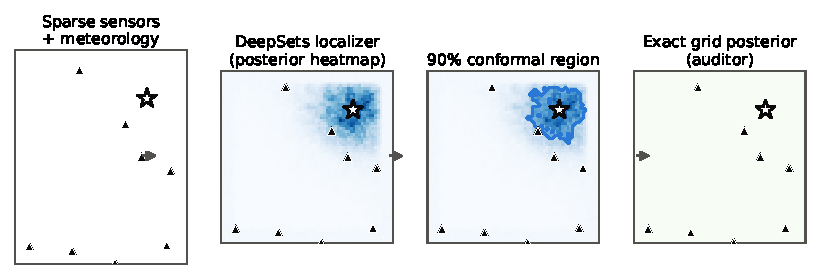
\includegraphics[width=\linewidth]{fig1_pipeline.pdf}
  \caption{\textbf{F1 --- Pipeline.} Sparse sensors plus meteorology feed the DeepSets localizer, which outputs
  a posterior heatmap; split conformal converts the heatmap into a $90\%$ region; the exact grid posterior
  serves as the auditor. Panels show a real median-difficulty test scenario (star = true source,
  triangles = sensors).}
  \label{fig:pipeline}
\end{figure}

\begin{figure}[h]
  \centering
  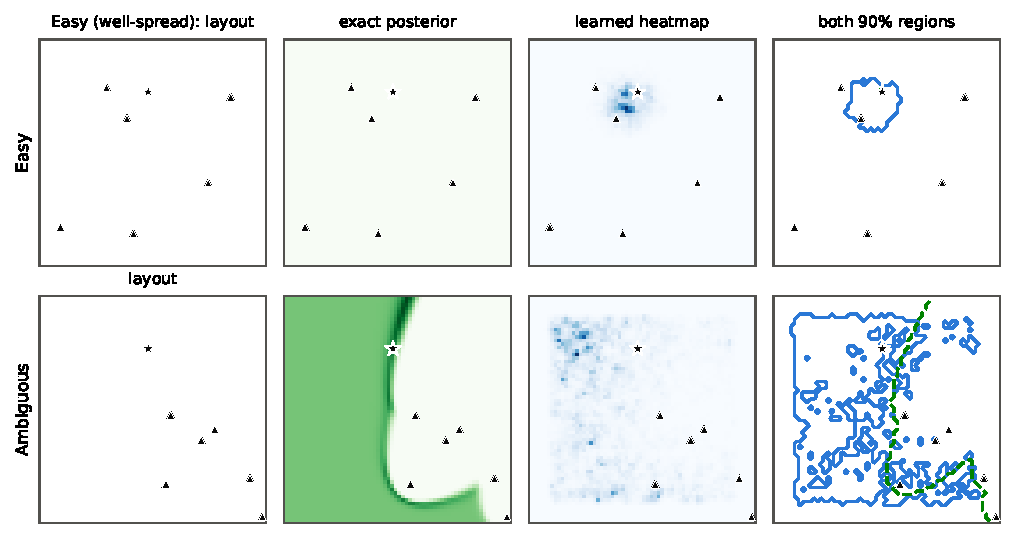
\includegraphics[width=\linewidth]{fig2_easy_vs_ambiguous.pdf}
  \caption{\textbf{F2 --- Easy vs.\ ambiguous scenario.} For an easy (well-spread sensors) and an ambiguous
  (confined-quadrant) scenario: sensor layout, exact posterior, learned heatmap, and both $90\%$ regions
  (solid blue = learned, dashed green = exact). The confined layout induces the directional ambiguity
  visible as the broad arc in the exact posterior.}
  \label{fig:scenarios}
\end{figure}

\section{Grid-Refinement Check}
\label{app:refine}

Recomputing the exact posterior on a $96 \times 96$ grid and re-running the identical conformal
procedure changes coverage by $-0.007$ ($0.9005$ vs.\ $0.9070$) and median area by $-0.006$
($0.0066$ vs.\ $0.0128$ as a domain fraction; finer cells resolve sharper regions), confirming the
$64 \times 64$ grid is adequate for the coverage claims. We ran this on the \emph{full} 2000-scenario
test split rather than the preregistered 100 scenarios: 100-scenario windows of the test split have
empirical coverage ranging from $0.79$ to $0.97$, so the 100-scenario version of this check cannot
resolve the effect it is looking for. Posterior normalization error at $96^2$: $1.4\times10^{-13}$.

\end{document}
